%%%%%%%%%%%%%%%%%%%%%%%%%%%%%%%%%%%%%%%%%%%%%%%%%%%%%%%%%%%%%%%%%%%%%
%                                                                   %
%	CHAPTER TWO, HARDWARE IN HPC                                    %
%                                                                   %
%%%%%%%%%%%%%%%%%%%%%%%%%%%%%%%%%%%%%%%%%%%%%%%%%%%%%%%%%%%%%%%%%%%%%

\chapter{Hardware in HPC}

\section{Introduction}

The knowledge of hardware architecture is essential to reach performances through optimizations.
Even if the nowadays software, API, framework or runtime already handle most of optimizations, the last percents of gain are architecture's dependent. 
In this chapter we describe the most important devices architectures from classical processors, General Purpose Graphics Processing Units (GPGPUs), Field Programmable Gate Arrays (FPGAs) and Application-Specific Integrated Circuits (ASICs).
This study keeps a focus on multi-core processors and GPUs as we based our tests on those devices. 

This chapter also details the architecture of some remarkable supercomputers. 
This has to go with the description of interconnection network with the most famous interconnection topologies. 

We choose to present the architectures in a chronological order following the models presented in the previous chapter with: SISD, MIMD and SIMD/SIMT and presenting the last released technologies.
We also present the optimizations of technologies with the arising of parallelism and new types of memories.

\section{Early improvements to Von Neumann machine}
In this section we present the different hardware from 1970s single core processors to nowadays multi-core and many-core architectures. 
We see the most important optimizations that are always implemented in the most recent machines like in/out of order processors, pre-fetching strategies, vectorization and the memory technologies. 
They are the milestones, the basic units, to build supercomputers. 

\subsection{Single core processors}
The first processors, around the 1970s, were built using a single computation core like described in the Von Neumann model. 
Many evolutions were made on those single cores processors from the memory, the order of instruction and the frequency.

\subsubsection{Transistor shrink and frequency}
\index{Frequency}
A lot of new ways to produce smaller transistors had been discovered from the 10$\mu m$ of 1971 to nowadays 10$nm$.
This allows the vendor to add more transistors on the same die, allowing more complex ISA and features for the CPU. 
%This will also be useful for the multi-core machine presented in the next part. 

In parallel of the shrink of transistors, the main feature for better performances with the single core architecture came from the frequency augmentation, the clock rate. 
Indeed, as fast as the clock rate get, more operations can be computed in a second on the core. 
In 1970s the frequency was about 4 MHz allowing a maximum of 4 millions of cycles per seconds. 
Nowadays core can work at a frequency of 4GHz and even 5GHz performing billions of operations per cycles. 

\subsubsection{In/Out-Of-Order} 
\index{In/Out of Order}
In-order-process is the one describes in previous chapter. 
The control unit fetches instruction in memory and the operands. The ALU computes the operation, and finally the result is stored in memory.

In this model the time to perform an instruction is the cumulation of: instruction fetching + operand(s) fetching + \textit{computation} + store the result.
This time can be high regarding the time when the ALU itself is busy for \textit{computation}, technically just one clock cycle. 
The idea of Out-of-order is to compute the instructions without following the Program Counter order. 
Indeed, for independent tasks (pointed out with dependency graphs) while the process fetches the next instructions data, the ALU can perform another operation with already available operands.
This leads to better usage of computational resources in the CPU and thus better overall performances. 

\subsubsection{Vectorization} 
\index{Vectorization}
\index{Unrolling}
\index{Loop tiling}
Vector processors allows the instructions to be executed at the same time in a SIMD manner. 
If the same instruction is executed on coalescent data they can be executed in the same clock cycle. 
We can, as an example, execute operations simultaneously on 4 to 8 floats with  a bus size of 128 or 256 bits in the same cycle.  
This tool requires specific care during coding with \textit{unrolling} and \textit{loop tiling} and will be address later in this study. 
The main downside on latest architectures is that vectorization slightly lower the frequency of processors to operate. 
This requires even more care during programming to avoid bad behavior leading to bad performances. 

\index{Cray-1}
The Cray-1 supercomputer\cite{russell1978cray}, installed in 1975 in the Los Alamos National Laboratory, is a perfect example of vector processor supercomputer.
This supercomputer was designed by Seymour Cray the founder of Cray Research.
Based on vector processor it was able to deliver up to 160 MFLops.
It was the fastest supercomputer of 1978 and due to its shape and price he was humorously called \textit{the world's most expansive love-seat}. 

\begin{figure}[t!]
\begin{center}
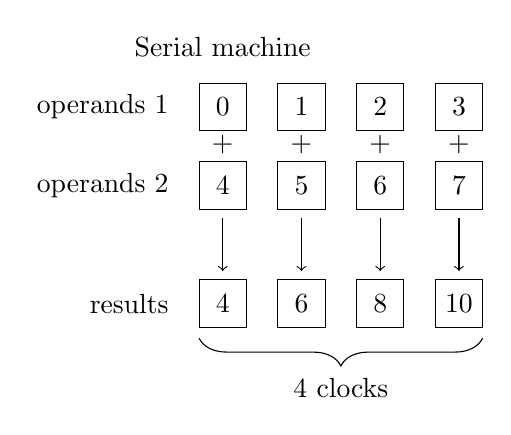
\begin{tikzpicture}
\foreach \x in {0,...,3}
{
	% Draw the rectangle 
	\draw (\x,0) rectangle (\x+.6,.6) node[pos=.5] (res\x) {
		\pgfmathparse{4+\x*2}
		\pgfmathprintnumber[precision=0]
        \pgfmathresult
    };
	\draw (\x,1.5) rectangle (\x+.6,2.1) node[pos=.5] (op2\x)  {
		\pgfmathparse{\x+4}
		\pgfmathprintnumber[precision=0]
        \pgfmathresult
    };
	\draw (\x,2.5) rectangle (\x+.6,3.1) node[pos=.5] (op1\x) {\x};
	% Draw the arrows for result
	\draw[->] ([yshift=-5pt]op2\x.south) -- ([yshift=5pt]res\x.north);
	\node at ([yshift=-7pt]op1\x.south) {$+$};
}
% add the arrow on top for clocks 
\draw [decorate,decoration={brace,amplitude=10pt,mirror,raise=4pt},yshift=0pt]
(0.,0) -- (3.6,0) node [black,midway,below,yshift=-15pt] {4 clocks};

\node[anchor=east] at ([xshift=-10pt]res0.west) {results};
\node[anchor=east] at ([xshift=-10pt]op10.west) {operands 1};
\node[anchor=east] at ([xshift=-10pt]op20.west) {operands 2};

\node[thick] at ([yshift=15pt]op10.north) {Serial machine};


% Add the name of architecture, classical serial 

% Add line name 
\end{tikzpicture}
\hspace{1cm}
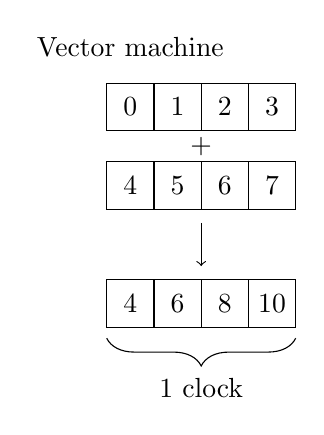
\begin{tikzpicture}
\foreach \x in {0,...,3}
{
	% Draw the rectangle 
	\draw (\x*.6,0) rectangle (\x*.6+.6,.6) node[pos=.5] (res\x) {
		\pgfmathparse{4+\x*2}
		\pgfmathprintnumber[precision=0]
        \pgfmathresult
    };
	\draw (\x*.6,1.5) rectangle (\x*.6+.6,2.1) node[pos=.5] (op2\x)  {
		\pgfmathparse{\x+4}
		\pgfmathprintnumber[precision=0]
        \pgfmathresult
    };
	\draw (\x*.6,2.5) rectangle (\x*.6+.6,3.1) node[pos=.5] (op1\x) {\x};
	% Draw the arrows for result
}

% Just onw arrow and plus sign 
\draw[->] ([yshift=-5pt]1.2,1.5) -- ([yshift=5pt]1.2,.6);
\node at ([yshift=-6pt]1.2,2.5) {$+$};

\draw [decorate,decoration={brace,amplitude=10pt,mirror,raise=4pt},yshift=0pt]
(0.,0) -- (2.4,0) node [black,midway,below,yshift=-15pt] {1 clock};

\node[thick] at ([yshift=15pt,]op10.north) {Vector machine};
\end{tikzpicture}
\end{center}
\caption{Vectorized processeur example on 4 integer addition: 128 bits wide bus}
\label{fig:2_HARD:vector}
\end{figure}

The behavior of vector machine is presented with a 16 bytes vector machine (4 integer of 4 bytes = 128 bits bus) on figure~\ref{fig:2_HARD:vector}. We see on left that performing the 4 operations requests 4 cycle and, at opposite, 1 cycle on the right with the vectorized machine.\\

Linked with the CPU optimizations, the memory optimizations also have to be considered. 
Indeed, even if the ALU can perform billions of operations per second it needs to be fed by fast transfers.

\subsubsection{Memory technology evolution}

The memories technologies optimizations contain several aspect. 
In early 1980s the augmentation of bus size from 4 bits, 8 bits, 16 bits for nowadays 32 bits for single precision and 64 bits for double precision. 
128 bits, 256 bits, etc. buses can also be find allowing technologies we just presented, vectorization. 
Different kind of technologies are considered: the SRAM and DRAM. 

\paragraph{SRAM: }
\index{Static Random Access Memory}
The Static Random Access Memory is built using so called "flip-flop" circuits that can store the data as long as the machine is powered. 
This kind of memory is very expensive to produce due to the number of transistor by memory cell needed and the size of the memory.
Therefore it is usually limited for small amount of storage. 
The SRAM is mainly used for cache memory. 
Cache is a memory mechanism that is useful to consider when targeting performance. 

\subparagraph{Cache memory: }
\index{Cache mechanism}
\begin{figure}[t!]
\centering
\begin{tikzpicture}
\node (rect) at (0,0) [draw,minimum width=2cm,minimum height=1cm] (cpu) {CPU};
\node[right = 1.5cm of cpu] (rect) [draw,minimum width=1cm,minimum height=.6cm] (cache_1) {Level 1};
\node[right = 1.2cm of cache_1] (rect) [draw,minimum width=1.5cm,minimum height=1cm] (cache_2) {Level 2};
\node[right = 1.8cm of cache_2] (rect) [draw,minimum width=1.5cm,minimum height=1.4cm] (cache_3) {Level 3};
\node[right = 1.5cm of cache_3] (rect) [draw,minimum width=4cm,minimum height=2.5cm] (ram) {Main memory};

\draw[thick,draw,red,dotted] (2.4,-1.2) rectangle  (10.1,1.2);
\node[below,red,thick] at (6.25,-1.2) {Cache}; 
% links 
\draw[->] ([yshift=5pt]cpu.east) -- ([yshift=5pt]cache_1.west);
\draw[<-] ([yshift=-5pt]cpu.east) -- ([yshift=-5pt]cache_1.west) node[midway,yshift=-10pt] {Fastest};

\draw[->] ([yshift=5pt]cache_1.east) -- ([yshift=5pt]cache_2.west);
\draw[<-] ([yshift=-5pt]cache_1.east) -- ([yshift=-5pt]cache_2.west) node[midway,yshift=-10pt] {Fast};

\draw[->] ([yshift=5pt]cache_2.east) -- ([yshift=5pt]cache_3.west);
\draw[<-] ([yshift=-5pt]cache_2.east) -- ([yshift=-5pt]cache_3.west) node[midway,yshift=-10pt] {Less fast};

\draw[->] ([yshift=5pt]cache_3.east) -- ([yshift=5pt]ram.west);
\draw[<-] ([yshift=-5pt]cache_3.east) -- ([yshift=-5pt]ram.west) node[midway,yshift=-10pt] {Slow};

\draw[<->,thick] (1,1.6) node[above]{Words} -- (12,1.6) node[above] {Blocks};
\node[above] at (6,1.6) {Transfer}; 
\end{tikzpicture}
\caption{Cache memory technology on three levels L1, L2 and L3}
\label{fig:2_HARD:caches}
\end{figure}

The main idea of cache technology is presented on figure~\ref{fig:2_HARD:caches}.
This little memory is built over several levels. 
The closer to the CPU is L1, then L2 and generally no more than L3 except on specific architecture. 
When looking for a data the CU will first check the L1 cache, otherwise L2 and L3 to get the data to higher level. 
From the main memory to the L3 cache \textit{blocks} are exchanged, they are chunks of memory. 
With the smaller level L2 and L1 line of informations usually called \textit{words} are exchanged.
This is based on the idea that if a data is used, it shall be use again in the near future.
Many cache architectures exist like direct, associative, fully associative, etc. 
In a program the ratio of cache accesses \textit{cache-hits} and \textit{cache-miss} respectively when a data is present in cache and when a data have to be retrieved from lower level or main memory can be very important to reach performances. 

\paragraph{DRAM: }
\index{Dynamic Random Access Memory}
The Dynamic Random Access Memory is based on transistors and capacitors to store the binary information.
This memory is less expansive to produce but needs to be refresh at a determined frequency however the data are lost. 
This refresh step is in fact a reading-writing operation on the whole memory at a specific frequency. 
There is several sub categories of DRAM used in different devices.

Depending on the way the bus are used we can find Single Data Rate, SDR, Double Data Rate, DDR and QDR, Quad Data Rates DRAM memories. 
The number of data carried can go from 1x to 4x but the limitation of those products is the price of memory constantly rising.  

\subsubsection{Pre-fetching} 
\index{Pre-fetching}
Based on memory optimization and especially the cache, pre-fecthing was developed.
When a data is not available in L1 cache, it has to be moved from either L2 to L1 or L3 to L2 to L1 or in the worst case RAM to L3 to L2 to L1. 
Pre-fecthing technology is a way to, knowing the next instructions operands, pre-fetch the data in closer cache. 
The pre-fetch can either be hardware or software implemented and can concern data and even instructions.

\subsection{Multi-core processors}
Around the beginning of 2000s the limitations of single core processors were too important. 
The frequency was already high and requested more power consumption and caused more heat dissipation. 
Unable to answer the constant augmentation of computational power needed for research and HPC, IBM was the first company to create a multi-core CPU in 2001, the Power4. 

The first idea was to provide multi-CPU devies, embedding several CPU on the same motherboard and allowing them to share memory. 
The evolution of that is multi-core, having several CPUs on the same die directly allowing more optimization inside the die combining all the advantages of single core processors.
We note here that in nowadays language the CPU, as describe in the Von Neumann model, is also the name of the die containing several CPUs. 
This is the architecture of most of nowadays processors. 
They are called multi-cores and provide up to 2 to 32 cores. 
Those processors are called "Host" because they are usually bootable and most of the accelerators need to be attached to them in order to work.

\begin{figure}
\centering 
\begin{tikzpicture}

\node (rect) at (0,0) [draw,minimum width=2cm,minimum height=1cm] (input) {Input Device};

\node[right = 1.5cm of input] (rect) [draw,minimum width=9cm,minimum height=5.1cm] (machine) {};

\node[fill=black!30] (rect) at ([yshift=-3.6cm]machine.north) [draw,minimum width=8.3cm,minimum height=.5cm] (l3) {Shared L3 Cache};

\foreach \x in {0,...,3}{
	\node[anchor=north west,fill=black!5] (rect) at ([yshift=-.2cm,xshift=\x*2.2cm+.2cm]machine.north west) [draw,minimum width=2cm,minimum height=1.9cm] (cpu\x) {};

	\node[anchor=north west,fill=white] (rect) at ([yshift=-.1cm,xshift=.1cm]cpu\x.north west) [draw,minimum width=1.8cm,minimum height=.5cm] {ALU};
	\node[anchor=north west,fill=white] (rect) at ([yshift=-.7cm,xshift=.1cm]cpu\x.north west) [draw,minimum width=1.8cm,minimum height=.5cm] {CU};
	\node[anchor=north west,fill=white] (rect) at ([yshift=-1.3cm,xshift=.1cm]cpu\x.north west) [draw,minimum width=1.8cm,minimum height=.5cm] {REG};
	% Cache memory
	\node[anchor=north west,fill=black!20] (rect) at ([yshift=-.3cm,xshift=.1cm]cpu\x.south west) [draw,minimum width=1.8cm,minimum height=.5cm] (l1\x) {L1/L2};
	% Arriw 
	\draw[->] ([xshift=-10pt]l1\x.north) -- ([xshift=-10pt]cpu\x.south);
	\draw[<-] ([xshift=10pt]l1\x.north) -- ([xshift=10pt]cpu\x.south);
	% Arrow to L3
	\draw[->] ([xshift=-10pt]l1\x.south) -- ([xshift=-10pt,yshift=-8pt]l1\x.south);
	\draw[<-] ([xshift=10pt]l1\x.south) -- ([xshift=10pt,yshift=-8pt]l1\x.south);

	%\draw[<-] ([xshift=10pt]l1\x.south) |- (l3.north);
	
}


\node[below = .3cm of l3] (rect) [draw,minimum width=8.3cm,minimum height=.7cm] (mem) {Main Memory};

\node[right = 1.5cm of machine] (rect) [draw,minimum width=2cm,minimum height=1cm] (output) {Output Device};

\draw[->] ([xshift=-10pt]mem.north) -- ([xshift=-10pt]l3.south);
\draw[<-] ([xshift=10pt]mem.north) -- ([xshift=10pt]l3.south);

\draw[->] (input.east) -- (machine.west);
\draw[->] (machine.east) -- (output.west);

\end{tikzpicture}
\caption{Multi-core CPU with 4 cores based on Von Neumann Model presented on figure~\ref{fig:2_HPC:von_neumann_model}}
\label{fig:2_HARD:von_neumann_model_multi-core}
\end{figure}

This architecture is presented on figure~\ref{fig:2_HARD:von_neumann_model_multi-core}.
The memory, like presented in the previous chapter, is now shared between the cores. 
The registers and cache are different: another layer is added to the cache and consistency have to be maintain over all the cores. 
If a process modify a data in the memory this information have to be spread over all the other users of this data, even in their local cache. 

%This new architecture model imposed new rules to consider the machine and especially their memory. 
%The cores on the same die need to have a concurrent access to the system memory to operate involving concurrent accesses and consistency problems.

\section{21th century architectures}
After years of developpement and research on hardware for Computer Science and specifically HPC, we present here the latest and best technologies to product efficient and general purpose supercomputers.

We present the latest architectures with multi-core, many-core and specific processors and the most famous vendors. 

\subsection{Multi-core}
The most world spread architecture in public and hight performance computing is the multi-core processors. 
Most of nowadays accelerators require a classical processor to offload tasks and data on it. 
We start from the most present processors in HPC world, the Intel company ones. 
We also present ARM which is another multi-core architecture base on RISC instructions set.

\subsubsection{Intel}
\index{Intel}
Intel was created in 1968 by a chemist and a physicists, Gordon E. Moore and Robert Noyce, in Mountain View, California. 
Nowadays processors are mostly Intel ones, this world leader equips around 90\% of the supercomputers (November 2017 TOP500 list).

In 2007 Intel adopted a production model called the "Tick Tock", presented on figure~\ref{fig:1_HPC:intel_tick_tock}.
\begin{figure}[t!]
\begin{center}
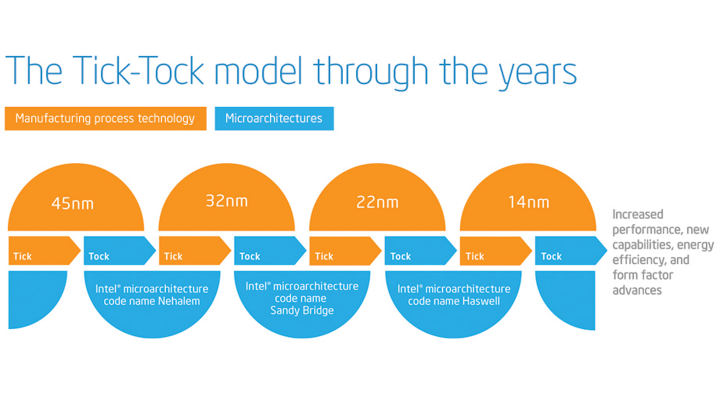
\includegraphics[width=.8\textwidth]{\locpath/figures/chap1/intel_tick_tock.png}
\caption{Intel Tick-Tock model}
\label{fig:1_HPC:intel_tick_tock}
\end{center}
\end{figure}
Since its creation this model followed the same fashion, a new manufacturing technology like shrink of the chip with better engraving on a "Tick" and a new micro-architecture delivered on a "Tock".
The Intel processors for HPC are called Xeon and features ECC memory, higher number of cores, large RAM support, large cache-memory, Hyper-threading, etc. compared to desktop processors. 
Every new processor have a code name. 
The last generations are chronologically called Westemere, Sandy Bridge, Ivy Bridge, Haswell, Broadwell, Skylake and Kaby lake. 
Kaby Lake, the last architecture of processor, does not exactly fit the usual "Tick-Tock" process because it is just based on optimizations of the Skylake architecture. 
It is produce like Skylake in 14nm.
This model seems to be hard to maintain due to the difficulties to engrave in less than 10nm with quantum tunneling. 
This leads to using more many-cores architecture and base next supercomputer generations on hybrid models. 

\paragraph{Hyper-threading}
\index{Hyper-threading}
Another specificity of Intel processor is Hyper-threading (HT). 
This technology makes a single physical processor appearing as two logical processors for user's level.
In fact a processor embedding 8 cores appears as a 16 cores for user. 
Adding more computation per node can technically allows the cores to switch context when data are fetched from the memory using the processor 100\% during all the computation. 
A lot of studies have been released on HT from Intel itself~\cite{marr2002hyperthreading} to other studies~\cite{bononi2006exploring,leng2002empirical}.
This optimization does not fit to all the cases and can be disable for normal use of the processors. 

\subsubsection{ARM}
\index{Advanced RISC architecture}
Back in 1980s, ARM stood for Acorn RISC Machine in reference of the first company implementing this kind of architecture, Acorn Computers. 
This company later changed the name to Advanced RISC Machine (ARM). 
ARM is a specific kind of processor based on RISC architecture as its ISA despite usual processors using CISC.
The downside of CISC machines makes them hard to create and they require way more transistor and thus energy to work. 
The ISA from the RISC is simpler and requires less transistors to operate and thus a smaller silicon area on the die.
Therefore, the energy required and the heat dissipated is less important. 
It would then be easier to create massively parallel processors based on ARM. 
On the other hand, simple ISA impose more work on the source compilation to fit the simple architecture. 
That makes the instructions sources longer and therefore more single instructions to execute. 

The ARM company provide several version of ARM processors named Cortex-A7X, Cortex-A5X and Cortex-A3X respectively balancing highest-performances, performances and efficiency and less power consumption. 
We find here the same kind of naming as Intel processors. 

\index{Mont-Blanc project}
The new ARMv8 architecture starts to have the tools to target HPC context~\cite{rico2017arm}.
The European approach towards energy efficient HPC, Mont-Blanc project\footnote{http://montblanc-project.eu/}, already constructs ARM based supercomputers. 
For the exascale project in Horizon 2020 this project focus on using ARM-based systems for HPC with many famous contributors with Atos/Bull as a project coordinator, ARM, French Alternative Energies and Atomic Energy Commission (CEA), Barcelona Supercomputing Center (BSC), etc.
The project is decomposed in several steps to finally reach exascale near 2020. 
The third step, Mont-Blanc 3, is about to work on a pre-exascale prototype powered by Cavium’s ThunderX2 ARM chip based on 64-bits ARMv8.

\subsection{Many-cores, SIMT}
\index{Single Instruction Multiple Threads}
Several architectures can be defined as many-cores. 
Those devices integrate thousands of cores that are usually control by less control units. 
We can consider those cores as "simpler" since they have to work synchronously and under the coordination of a control unit.
They are based on SIMD Flynn taxonomy. 
Some devices are specific like the Xeon Phi of Intel integrating a hundred of regular processor cores which can work independently. 

\subsubsection{GPU}
\index{Graphics Processing Unit}
When a CPU can usually have 2 to 32 computation cores that can operate on different instruction streams, the SIMT architecture of the GPU is slightly different. 
The cores are grouped and have to share the same instruction at the same clock time but all the groups can have their own instruction. 

\begin{figure}
\begin{center}
% classical processor
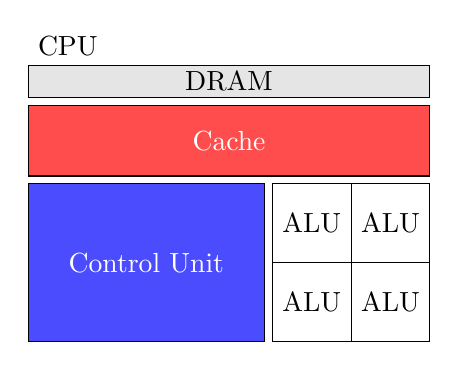
\begin{tikzpicture}
% ALUs
\foreach \x in {3,...,4}
	\foreach \y in {0,...,1}
		\draw[] (\x+.1,\y) rectangle (\x+1.1,\y+1) node[pos=.5] {ALU};
% Control Unit
\draw[fill=blue!70] (0,0) rectangle (3,2) node[pos=.5,text=white] {Control Unit};
%Cache
\draw[fill=red!70] (0,2.1) rectangle (5.1,3) node[pos=.5,text=white] {Cache};
% DRAM
\draw[fill=black!10] (0,3.1) rectangle (5.1,3.5) node[pos=.5] {DRAM};
%Name 
\node[yshift=7pt,anchor=west] at (0,3.5) {CPU};
\end{tikzpicture}
\hspace{1cm}
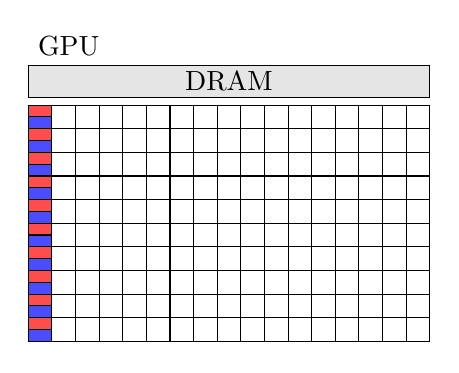
\begin{tikzpicture}
% ALUs
\foreach \y in {0,...,9}
{
	\draw[fill=blue!70] (0,\y * .3) rectangle (.3,\y * .3 + .15) node[pos=.5] {};
	\draw[fill=red!70] (0,\y * .3 + .15) rectangle (.3,\y * .3 + .3) node[pos=.5] {};
	\foreach \x in {1,...,16}
		\draw[] (\x*.3,\y*.3) rectangle (\x *.3+.3,\y*.3+.3) node[pos=.5] {};
}
% DRAM
\draw[fill=black!10] (0,3.1) rectangle (5.1,3.5) node[pos=.5] {DRAM};
% Name 
\node[yshift=7pt,anchor=west] at (0,3.5) {GPU};
\end{tikzpicture}
\end{center}
\caption{Multi-core versus Many-core architecture, case of GPUs}
\label{fig:2_HARD:gpu}
\end{figure}

Figure~\ref{fig:2_HARD:gpu} present the vision between CPU and GPU processors. 
We see on that figure the usual topology with the ALU lined up in front of their control unit and shared cache memory. 
Every ALU also have its own memory and registers to operate local computations. 

Those devices are called General Purpose Graphics Processing Units (GPGPUs). 
They are derivative from classical GPUs used for graphics purpose.
Pioneer shows that they can be use efficiently for classical scientific computations.
The vendor provides then specific GPU for general purpose computing.  
We present here the two main companies providing GPGPUs for HPC world: NVIDIA and AMD.

\paragraph{NVIDIA GPU architecture}
\index{NVIDIA}
The NVIDIA company was fonded in April 1993 in Santa Clara, Carolina, by three persons in which Jensen Huang, the actual CEO.
The company name seems to come from \textit{invidia} the Latin word for Envy and vision for graphics rendering. 

Known as the pioneer in graphics, cryptocurrency, portable devices and now Artificial Intelligence (IA), it seems to be even the creator of the name "GPU".
NVIDIA's GPUs, inspired from visualization and gaming at a first glance, are available as a dedicated device for HPC purpose since the company released the brand named \textit{Tesla}. 
The public GPUs can also be use for dedicated computation but does not feature ECC memory, double precision or special functions/FFT cores. 
The different versions of the architecture are named following famous physicists, chronologically: Tesla, Fermi, Kepler, Maxwell, Pascal and Volta.

\index{K20Xm}
We describe here the Kepler brand GPU and more specifically the K20Xm GPU on which we based our study. 
\begin{figure}
\centering
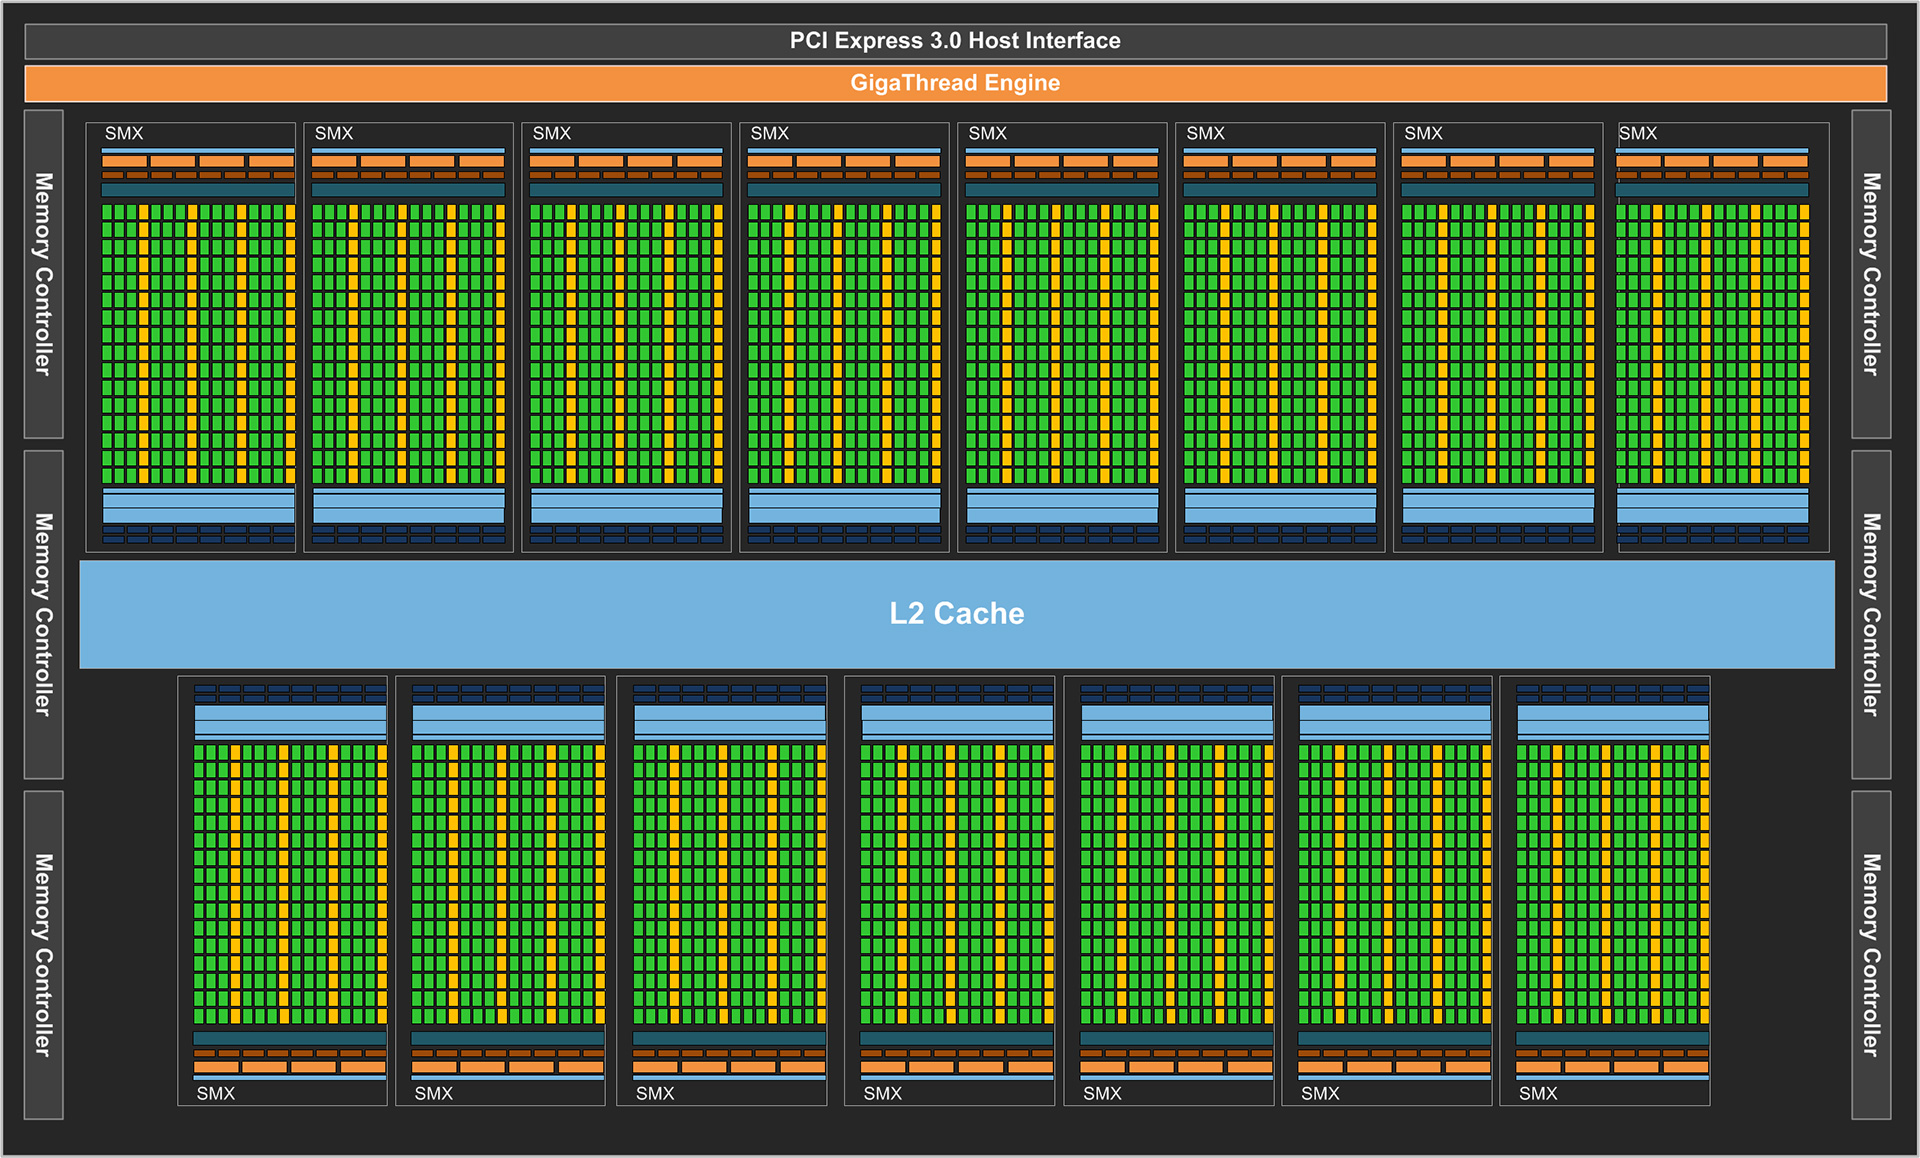
\includegraphics[width=\textwidth]{\locpath/figures/chap1/kepler_architecture.jpeg}
\caption{NVIDIA Tesla Kepler architecture. Single-precision in green and double-precision in yellow}
\label{fig:2_HARD:kepler_arch}
\end{figure}
This NVIDIA Tesla Kepler GPU is based on the GK110 graphics processor describes in the white-paper\cite{nvidia2012nvidias} on 28nm process.
The figure~\ref{fig:2_HARD:kepler_arch} is a representation of the physical elements of this graphics processor. 
The K20X comes in active and passive cooling mode with respectively K20Xc and K20Xm.
This GPU embeds 2688 CUDA cores distributed in 14 SMX (we note that GK110 normally provides 15 SMX but only 14 are present  on the K20X).
In this model each SMX contains 192 single precisions cores, 64 double precision cores, 32 special function units and 32 load/store units.
In a SMX the memory provides 65536 32-bits registers, 64KB of shared memory L1 cache, 48KB of read-only cache
The L2 cache is 1546KB shared by the SMX for a total of 6GB of memory adding the DRAM.
The whole memory is protected using Single‐Error Correct Double‐Error Detect (SECDED) ECC code.
The power consumption is estimated to 225W.
This GPGPU is expected to produce 1.31 TFLOPS for double-precision and 3.95 TFLOPS of single-precision.

\paragraph{AMD}
\index{AMD}
Another company is providing GPUs for HPC, Advanced Micro Devices (AMD). 
In front of the huge success of NVIDIA GPU that leads from far the HPC market, it is hard for AMD to find a place for its GPGPUs in HPC. 
Their HPC GPUs are called FirePro.
They are targeted using a language near CUDA but not hold by a single company called OpenCL. 
An interesting creation of AMD is the Accelerated Processing Units (APUs) which embedded the processor and the GPU on the same die since 2011. 
This solution allows them to target the same memory. 

In the race to market and performances, AMD found a accord with Intel to provide dies featuring Intel processor, AMD GPU and common HBM memory. 
The project is call  Kaby Lake-G and announce for first semester of 2018 but for public, not HPC itself. 

\subsubsection{Intel Xeon Phi}
\index{Xeon Phi}
Another specific HPC product from Intel is the Xeon Phi. 
This device can be considered as a Host or Device/Accelerator machine. 
Intel describes it as "a bootable host processor that delivers massive parallelism and vectorization".
This architecture embedded multiple multi-cores processors interconnected. 
This is call Intel's Many Integrated Core (MIC).
The architectures names are Knights Ferry, Knights Corner and Knight Landing~\cite{sodani2016knights}. 
The last architecture, Knight Hill, was recently canceled by Intel due to low performances and to focus the Xeon Phi for Exascale.
The main advantage of this architecture compared to GPGPUs is the x86 compatibility of the embedded cores and the fact this device can boot and use to drive other accelerators. 
They also feature more complex operations and handle double precision natively.
We considered the Xeon Phi in the many-cores architecture despite the fact that it is composed of completely independent processors. 
This is due to the number of cores that is very high and the fact it can be use as an accelerator instead of the host.  


\subsubsection{PEZY}
\index{PEZY}
Another many-core architecture just appears in the last benchmarks. 
The PEZY Super Computer 2, PEZY-SC2, is the third many-core microprocessor developed by the company PEZY. 
The three first machine ranked in the GREEN500 list are accelerator using this many-core die. 
We also note that in the November 2017 list the 4th supercomputer, Gyoukou, is also powered by PEZY-SC2 cards.

\subsection{Other architectures}
Numerous architecture have not been presented because out of scope in this study. 
We present here two technologies we have been confronted in our researches and that can be tomorrow solution for exascale in HPC. 
\subsubsection{FPGA}
\index{Field Programmable Gates Array}
Field Programmable Gates Array are device that can be reprogram to fit the needs of the user after their construction.
The leader was historically Altera with the Stratix, Arria and Cyclone FPGAs and is now part of Intel. 
With the FPGAs the user have access to the hardware itself and can design its own circuit. 
Nowadays FPGA can be targeted with OpenCL programming language. 
The arrival of Intel in this market promises the best hopes for HPC version of FPGAs. 
The main gap for users is the circuit building itself, perfect to respond to specific needs but hard to setup. 
\subsubsection{ASIC}
\index{Application Specified Integrated Circuits}
Application Specified Integrated Circuits are dedicated device construct for on purpose. 
An example of ASIC can be the Gravity Pipe (GRAPE) which is dedicated to compute gravitation given mass/positions.
Google leads the way for ASIC and just created its dedicated devices to boost AI bots.
We also find ASIC in some optimized communication devices like in fast interconnection network in HPC.  

\section{Distributed architectures}

The technologies presented in previous part is the milestone of supercomputers. 
They are used together in a whole system to create machine delivering incredible computational power.

\subsection{Architecture of a supercomputer}
From the hardware described before we can create the architecture of a cluster from the smallest unit, cores, nodes, to the whole system: 

\begin{description}[noitemsep,nolistsep]
\item[Core:] A core is the smallest unit in our devices. 
It can refer to the Von Neumann model in case of core with ALU and CU. 
We can separate core from CPU to GPU, the first one able to be independent whereas the second ones working together and sharing the same program counter. 
\item[Socket/Host:] A socket is mistakenly called a CPU in nowadays language. It is, for multi-cores sockets, composed of several cores. The name Host comes from the Host-Device architecture using accelerators. 
\item[Accelerators/Devices:] Accelerators are devices that, when attached to the Host, provide additional computational power. 
We can identify them as GPUs, FPGAs, ASICs, etc. 
A socket can have access to one or more accelerators.
They can also share the accelerator usage. 
\item[Computation node: ] The next layer of our HPC system if the computation node. Grouping together several socket and accelerators sharing memory;
\item[Rack: ] A rack is a set of computation nodes, generally a vertical stack. 
It can also include specific nodes dedicated to the network or the Input/Output.
\item[Interconnection: ] The nodes are grouped together with hard wire connection following a specific interconnection topology with very high bandwidth.
\item[System/Cluster/Supercomputer] The cluster group several racks though an interconnection network.
\end{description}

In order to connect node together and allow distributed programming an interconnect technology is required. 
Interconnection network is the way the nodes of a cluster are connected together. 

\subsection{Interconnection topologies}
\index{Interconnect}
Several topologies exists from point to point to multi dimensional torus.
%
\begin{figure}[t!]
\centering
\resizebox {.14\columnwidth} {!} {
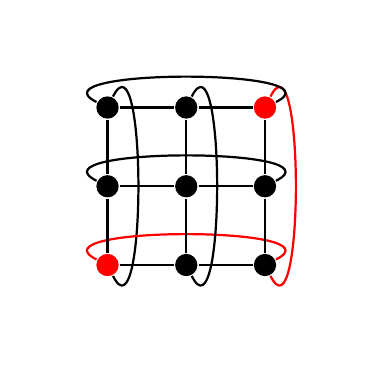
\begin{tikzpicture}[thick,inner sep=0.1cm]
	\node [fill,circle,red] (node 1000) at (0,0) {};
	\node [fill,circle] (node 1001) at (1,0) {};
	\node [fill,circle] (node 1002) at (2,0) {};
	\node [fill,circle] (node 1003) at (0,1) {};
	\node [fill,circle] (node 1004) at (1,1) {};
	\node [fill,circle] (node 1005) at (2,1) {};
	\node [fill,circle] (node 1006) at (0,2) {};
	\node [fill,circle] (node 1007) at (1,2) {};
	\node [fill,circle,red] (node 1008) at (2,2) {};
	
	\draw (node 1000)
							         .. controls +(0.500000,-1.000000)
							                 and +(0.500000,1.000000)
							         .. (node 1006);
	\draw[red] (node 1000)
							         .. controls +(-1.000000,0.500000)
							                 and +(1.000000,0.500000)
							         .. (node 1002);
	\draw (node 1000) -- (node 1001);
	\draw (node 1000) -- (node 1003);
	\draw (node 1001) -- (node 1004);
	\draw (node 1001)
							         .. controls +(0.500000,-1.000000)
							                 and +(0.500000,1.000000)
							         .. (node 1007);
	\draw (node 1002) -- (node 1005);
	\draw (node 1002) -- (node 1001);
	\draw[red] (node 1002)
							         .. controls +(0.500000,-1.000000)
							                 and +(0.500000,1.000000)
							         .. (node 1008);
	
	\draw (node 1003)
							         .. controls +(-1.000000,0.500000)
							                 and +(1.000000,0.500000)
							         .. (node 1005);
	\draw (node 1003) -- (node 1006);
	\draw (node 1003) -- (node 1004);
	\draw (node 1004) -- (node 1005);
	\draw (node 1004) -- (node 1007);
	\draw (node 1005) -- (node 1008);
	\draw (node 1006)
							         .. controls +(-1.000000,0.500000)
							                 and +(1.000000,0.500000)
							         .. (node 1008);
	\draw (node 1006) -- (node 1007);
	\draw (node 1007) -- (node 1008);
\end{tikzpicture}
}
%\vspace{1cm}
\resizebox {.34\columnwidth} {!} {
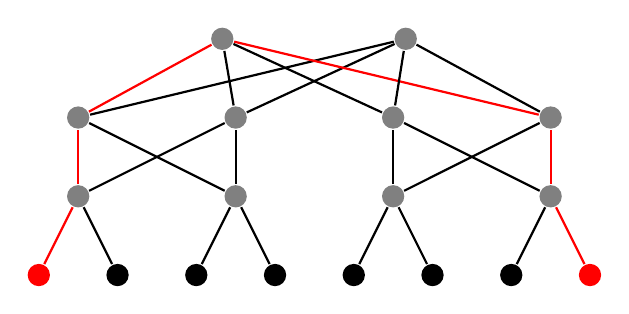
\begin{tikzpicture}[thick,inner sep=0.1cm]
	
	\node [fill,circle,red] (node a) at (0,0) {};
	\node [fill,circle] (node b) at (1,0) {};
	\node [fill,circle] (node c) at (2,0) {};
	\node [fill,circle] (node d) at (3,0) {};
	\node [fill,circle] (node e) at (4,0) {};
	\node [fill,circle] (node f) at (5,0) {};
	\node [fill,circle] (node g) at (6,0) {};
	\node [fill,circle,red] (node h) at (7,0) {};

	\node [fill,circle,black!50] (node a0) at (0.5,1) {};
	\node [fill,circle,black!50] (node a1) at (2.5,1) {};
	\node [fill,circle,black!50] (node a2) at (4.5,1) {};
	\node [fill,circle,black!50] (node a3) at (6.5,1) {};
	\node [fill,circle,black!50] (node a4) at (0.5,2) {};
	\node [fill,circle,black!50] (node a5) at (2.5,2) {};
	\node [fill,circle,black!50] (node a6) at (4.5,2) {};
	\node [fill,circle,black!50] (node a7) at (6.5,2) {};

	\node [fill,circle,black!50] (node n0) at (2.33,3) {};
	\node [fill,circle,black!50] (node n1) at (4.66,3) {};

	\draw[red] (node a) -- (node a0);
	\draw (node b) -- (node a0);
	\draw (node c) -- (node a1);
	\draw (node d) -- (node a1);
	\draw (node e) -- (node a2);
	\draw (node f) -- (node a2);
	\draw (node g) -- (node a3);
	\draw[red] (node h) -- (node a3);

	\draw[red] (node a0) -- (node a4);
	\draw (node a0) -- (node a5);
	\draw (node a1) -- (node a4);
	\draw (node a1) -- (node a5);
	\draw (node a2) -- (node a6);
	\draw (node a2) -- (node a7);
	\draw (node a3) -- (node a6);
	\draw[red] (node a3) -- (node a7);

	\draw[red] (node n0) -- (node a4);
	\draw (node n1) -- (node a5);
	\draw (node n0) -- (node a5);
	\draw (node n1) -- (node a4);
	\draw (node n0) -- (node a6);
	\draw (node n1) -- (node a7);
	\draw[red] (node n0) -- (node a7);
	\draw (node n1) -- (node a6);
\end{tikzpicture}
}
%\caption{Torus and 4-ary tree}
%\end{figure}
%\begin{figure}
\resizebox {.24\columnwidth} {!} {
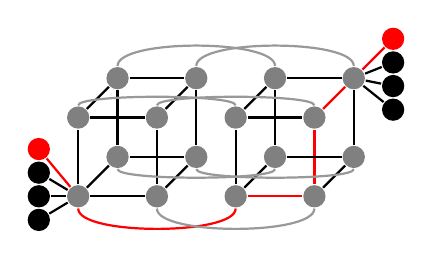
\begin{tikzpicture}[thick,inner sep=0.1cm]
	
	\node [fill,circle,black!50] (node a0) at (0,0) {};
	\node [fill,circle,black!50] (node b0) at (1,0) {};
	\node [fill,circle,black!50] (node c0) at (0,1) {};
	\node [fill,circle,black!50] (node d0) at (1,1) {};
	\node [fill,circle,black!50] (node e0) at (0.5,0.5) {};
	\node [fill,circle,black!50] (node f0) at (1.5,0.5) {};
	\node [fill,circle,black!50] (node g0) at (0.5,1.5) {};
	\node [fill,circle,black!50] (node h0) at (1.5,1.5) {};

	\node [fill,circle,black!50] (node a1) at (2,0) {};
	\node [fill,circle,black!50] (node b1) at (3,0) {};
	\node [fill,circle,black!50] (node c1) at (2,1) {};
	\node [fill,circle,black!50] (node d1) at (3,1) {};
	\node [fill,circle,black!50] (node e1) at (2.5,0.5) {};
	\node [fill,circle,black!50] (node f1) at (3.5,0.5) {};
	\node [fill,circle,black!50] (node g1) at (2.5,1.5) {};
	\node [fill,circle,black!50] (node h1) at (3.5,1.5) {};

	\node [fill,circle,red] (node cn0) at (4,2.) {};
	\node [fill,circle] (node cn1) at (4,1.7) {};
	\node [fill,circle] (node cn2) at (4,1.4) {};
	\node [fill,circle] (node cn3) at (4,1.1) {};

	\node [fill,circle] (node cn4) at (-0.5,-0.3) {};
	\node [fill,circle] (node cn5) at (-0.5,0.0) {};
	\node [fill,circle] (node cn6) at (-0.5,0.3) {};
	\node [fill,circle,red] (node cn7) at (-0.5,0.6) {};


	\draw (node a0) -- (node b0);
	\draw (node b0) -- (node d0);
	\draw (node c0) -- (node d0);
	\draw (node a0) -- (node c0);
	\draw (node e0) -- (node f0);
	\draw (node f0) -- (node h0);
	\draw (node g0) -- (node h0);
	\draw (node e0) -- (node g0);

	\draw (node a0) -- (node e0);
	\draw (node b0) -- (node f0);
	\draw (node c0) -- (node g0);
	\draw (node d0) -- (node h0);

	\draw[red] (node a1) -- (node b1);
	\draw[red] (node b1) -- (node d1);
	\draw (node c1) -- (node d1);
	\draw (node a1) -- (node c1);
	\draw (node e1) -- (node f1);
	\draw (node f1) -- (node h1);
	\draw (node g1) -- (node h1);
	\draw (node e1) -- (node g1);

	\draw (node a1) -- (node e1);
	\draw (node b1) -- (node f1);
	\draw (node c1) -- (node g1);
	\draw[red] (node d1) -- (node h1);

	\draw[red] (node cn0) -- (node h1);
	\draw (node cn1) -- (node h1);
	\draw (node cn2) -- (node h1);
	\draw (node cn3) -- (node h1);
	\draw (node cn4) -- (node a0);
	\draw (node cn5) -- (node a0);
	\draw (node cn6) -- (node a0);
	\draw[red] (node cn7) -- (node a0);

	%\draw (node a0) -- (node a1);
	\draw[red] (node a0)
		        .. controls +(0.,-0.500000)
		                 and +(0.,-0.500000)
		        .. (node a1);
	\draw[black!40] (node b0) 
				.. controls +(0.,-0.500000)
		                 and +(0.,-0.500000)
		        .. (node b1);
	\draw[black!40] (node c0) 
				.. controls +(0.,0.300000)
		                 and +(0.,0.300000)
		        ..  (node c1);
	\draw[black!40] (node d0) 
				.. controls +(0.,0.300000)
		                 and +(0.,0.300000)
		        ..  (node d1);
	\draw[black!40] (node e0) 
				.. controls +(0.,-0.300000)
		                 and +(0.,-0.300000)
		        ..  (node e1);
	\draw[black!40] (node f0) 
				.. controls +(0.,-0.300000)
		                 and +(0.,-0.300000)
		        ..  (node f1);
	\draw[black!40] (node g0) 
				.. controls +(0.,0.500000)
		                 and +(0.,0.500000)
		        ..  (node g1);
	\draw[black!40] (node h0) 
				.. controls +(0.,0.500000)
		                 and +(0.,0.500000)
		        ..  (node h1);
\end{tikzpicture}
}
%\hspace{1cm}
\resizebox {.24\columnwidth} {!} {
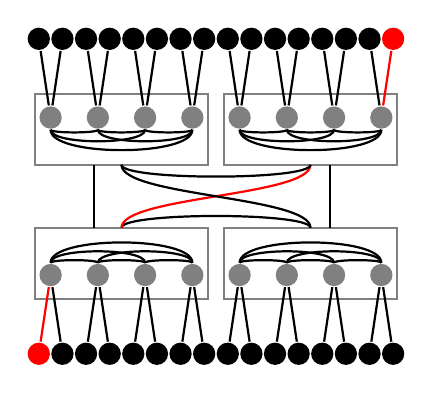
\begin{tikzpicture}[thick,inner sep=0.1cm]
	\node [fill,circle,black!50] (node a00) at (0.45,1) {};
	\node [fill,circle,black!50] (node a01) at (1.05,1) {};
	\node [fill,circle,black!50] (node a02) at (1.65,1) {};
	\node [fill,circle,black!50] (node a03) at (2.25,1) {};
	\node [fill,circle,red] (node n01) at (0.3,0) {};
	\node [fill,circle] (node n02) at (0.6,0) {};
	\node [fill,circle] (node n03) at (0.9,0) {};
	\node [fill,circle] (node n04) at (1.2,0) {};
	\node [fill,circle] (node n05) at (1.5,0) {};
	\node [fill,circle] (node n06) at (1.8,0) {};
	\node [fill,circle] (node n07) at (2.1,0) {};
	\node [fill,circle] (node n08) at (2.4,0) {};

	\node [fill,circle,black!50] (node a10) at (2.85,1) {};
	\node [fill,circle,black!50] (node a11) at (3.45,1) {};
	\node [fill,circle,black!50] (node a12) at (4.05,1) {};
	\node [fill,circle,black!50] (node a13) at (4.65,1) {};
	\node [fill,circle] (node n11) at (2.7,0) {};
	\node [fill,circle] (node n12) at (3,0) {};
	\node [fill,circle] (node n13) at (3.3,0) {};
	\node [fill,circle] (node n14) at (3.6,0) {};
	\node [fill,circle] (node n15) at (3.9,0) {};
	\node [fill,circle] (node n16) at (4.2,0) {};
	\node [fill,circle] (node n17) at (4.5,0) {};
	\node [fill,circle] (node n18) at (4.8,0) {};

	\node [fill,circle,black!50] (node a20) at (0.45,3) {};
	\node [fill,circle,black!50] (node a21) at (1.05,3) {};
	\node [fill,circle,black!50] (node a22) at (1.65,3) {};
	\node [fill,circle,black!50] (node a23) at (2.25,3) {};
	\node [fill,circle] (node n21) at (0.3,4) {};
	\node [fill,circle] (node n22) at (0.6,4) {};
	\node [fill,circle] (node n23) at (0.9,4) {};
	\node [fill,circle] (node n24) at (1.2,4) {};
	\node [fill,circle] (node n25) at (1.5,4) {};
	\node [fill,circle] (node n26) at (1.8,4) {};
	\node [fill,circle] (node n27) at (2.1,4) {};
	\node [fill,circle] (node n28) at (2.4,4) {};

	\node [fill,circle,black!50] (node a30) at (2.85,3) {};
	\node [fill,circle,black!50] (node a31) at (3.45,3) {};
	\node [fill,circle,black!50] (node a32) at (4.05,3) {};
	\node [fill,circle,black!50] (node a33) at (4.65,3) {};
	\node [fill,circle] (node n31) at (2.7,4) {};
	\node [fill,circle] (node n32) at (3,4) {};
	\node [fill,circle] (node n33) at (3.3,4) {};
	\node [fill,circle] (node n34) at (3.6,4) {};
	\node [fill,circle] (node n35) at (3.9,4) {};
	\node [fill,circle] (node n36) at (4.2,4) {};
	\node [fill,circle] (node n37) at (4.5,4) {};
	\node [fill,circle,red] (node n38) at (4.8,4) {};

	\draw[black!50] (2.65,2.4) rectangle (4.85,3.3);
	\draw[black!50] (0.25,2.4) rectangle (2.45,3.3);

	\draw[black!50] (2.65,0.7) rectangle (4.85,1.6);
	\draw[black!50] (0.25,0.7) rectangle (2.45,1.6);

	\draw (1.35,1.6)
	.. controls +(0.,0.2)
	    and +(0.,0.2)
	..  (3.75,1.6); 

	\draw[red] (1.35,1.6)
	.. controls +(0.,0.4)
	    and +(0.,-0.4)
	..  (3.75,2.4); 
	%\draw (1.35,1.6) -- (3.75,2.4);
	\draw (3.75,1.6)
	.. controls +(0.,0.4)
	    and +(0.,-0.4)
	..  (1.35,2.4); 
	%\draw (3.75,1.6) -- (1.35,2.4);

	\draw (1.,1.6) -- (1.,2.4);
	\draw (4.,1.6) -- (4.,2.4);

	\draw (1.35,2.4)
	.. controls +(0.,-0.2)
	    and +(0.,-0.2)
	..  (3.75,2.4); 


	\draw[red] (node n01) -- (node a00);
	\draw (node n02) -- (node a00);
	\draw (node n03) -- (node a01);
	\draw (node n04) -- (node a01);
	\draw (node n05) -- (node a02);
	\draw (node n06) -- (node a02);
	\draw (node n07) -- (node a03);
	\draw (node n08) -- (node a03);

	\draw (node n11) -- (node a10);
	\draw (node n12) -- (node a10);
	\draw (node n13) -- (node a11);
	\draw (node n14) -- (node a11);
	\draw (node n15) -- (node a12);
	\draw (node n16) -- (node a12);
	\draw (node n17) -- (node a13);
	\draw (node n18) -- (node a13);

	\draw (node n21) -- (node a20);
	\draw (node n22) -- (node a20);
	\draw (node n23) -- (node a21);
	\draw (node n24) -- (node a21);
	\draw (node n25) -- (node a22);
	\draw (node n26) -- (node a22);
	\draw (node n27) -- (node a23);
	\draw (node n28) -- (node a23);

	\draw (node n31) -- (node a30);
	\draw (node n32) -- (node a30);
	\draw (node n33) -- (node a31);
	\draw (node n34) -- (node a31);
	\draw (node n35) -- (node a32);
	\draw (node n36) -- (node a32);
	\draw (node n37) -- (node a33);
	\draw[red] (node n38) -- (node a33);

	\draw (node a00) 
	.. controls +(0.,0.2)
	    and +(0.,0.2)
	..  (node a01);
	\draw (node a00) 
	.. controls +(0.,0.35)
	    and +(0.,0.35)
	..  (node a02);
	\draw (node a00) 
	.. controls +(0.,0.5)
	    and +(0.,0.5)
	..  (node a03);
	\draw (node a01) 
	.. controls +(0.,0.2)
	    and +(0.,0.2)
	..  (node a02);
	\draw (node a01) 
	.. controls +(0.,0.35)
	    and +(0.,0.35)
	..  (node a03);
	\draw (node a02) 
	.. controls +(0.,0.2)
	    and +(0.,0.2)
	..  (node a03);

	\draw (node a10) 
	.. controls +(0.,0.2)
	    and +(0.,0.2)
	..  (node a11);
	\draw (node a10) 
	.. controls +(0.,0.35)
	    and +(0.,0.35)
	..  (node a12);
	\draw (node a10) 
	.. controls +(0.,0.5)
	    and +(0.,0.5)
	..  (node a13);
	\draw (node a11) 
	.. controls +(0.,0.2)
	    and +(0.,0.2)
	..  (node a12);
	\draw (node a11) 
	.. controls +(0.,0.35)
	    and +(0.,0.35)
	..  (node a13);
	\draw (node a12) 
	.. controls +(0.,0.2)
	    and +(0.,0.2)
	..  (node a13);

	\draw (node a20) 
	.. controls +(0.,-0.2)
	    and +(0.,-0.2)
	..  (node a21);
	\draw (node a20) 
	.. controls +(0.,-0.35)
	    and +(0.,-0.35)
	..  (node a22);
	\draw (node a20) 
	.. controls +(0.,-0.5)
	    and +(0.,-0.5)
	..  (node a23);
	\draw (node a21) 
	.. controls +(0.,-0.2)
	    and +(0.,-0.2)
	..  (node a22);
	\draw (node a21) 
	.. controls +(0.,-0.35)
	    and +(0.,-0.35)
	..  (node a23);
	\draw (node a22) 
	.. controls +(0.,-0.2)
	    and +(0.,-0.2)
	..  (node a23);

	\draw (node a30) 
	.. controls +(0.,-0.2)
	    and +(0.,-0.2)
	..  (node a31);
	\draw (node a30) 
	.. controls +(0.,-0.35)
	    and +(0.,-0.35)
	..  (node a32);
	\draw (node a30) 
	.. controls +(0.,-0.5)
	    and +(0.,-0.5)
	..  (node a33);
	\draw (node a31) 
	.. controls +(0.,-0.2)
	    and +(0.,-0.2)
	..  (node a32);
	\draw (node a31) 
	.. controls +(0.,-0.35)
	    and +(0.,-0.35)
	..  (node a33);
	\draw (node a32) 
	.. controls +(0.,-0.2)
	    and +(0.,-0.2)
	..  (node a33);
\end{tikzpicture}
}
\caption{Torus, Fat-Tree, HyperX, DragonFly}
\label{fig:1_HPC:topology}
\end{figure}
%
The figure~\ref{fig:1_HPC:topology} is a representation of famous topologies. 
Each interconnect technology has its own specificity. 
These networks takes in account the number of nodes to interconnect and the targeted bandwidth/budget.
Several declination of each network are not detailed here. 
The Mesh and the Torus are use as a basis in lower layers of others more complex interconnection networks. 
A perfect example is the supercomputer called K-Computer describe in the next section.
The Fat Tree presented here is a k-ary Fat Tree, higher the position in the tree more connection are found and the bandwidth is important. The nodes are available as the leafs, on the middle level we find the switches and on top the routers. 
Another topology, HyperX\cite{ahn2009hyperx}, is base on Hyper-Cube.
The DragonFly\cite{kim2008technology} interconnect is recent, 2008, and use in nowadays supercomputers.

InfiniBand (IB)\index{Infiniband} is the most spread technology used for interconnect with different kind of bandwidth presented in figure~\ref{fig:1_HPC:infiniband}.
It provides high bandwidth and small latency and companies like Intel, Mellanox, etc provide directly adapters and switches specifically for IB. 

\begin{table}[t!]
\begin{center}
\[\arraycolsep=0.pt\def\arraystretch{1.2}
\begin{tabular}{| l | l | l || l | l | l | }
\hline
\textbf{Name} & \textbf{Gbs} & \textbf{Year} & \textbf{Name} & \textbf{Gbs} & \textbf{Year} \\
\hline
\hline
Single DR & 2.5 & 2003 & Enhanced DR & 25 & 2014 \\
\hline
Double DR & 5 & 2005 & Highg DR & 50 & 2017 \\
\hline
Quad DR & 10 & 2007 & Next DR & 100 & 2020 \\
\hline
Fourth DR & 14 & 2011 & & &  \\
\hline
\end{tabular}
\]
\caption{InfiniBand technologies name, year and bandwidth}
\label{fig:1_HPC:infiniband}
\end{center}
\end{table}

Unfortunately this  augmentation of clock rate is not sustainable due to the energy required and the heat generated by the running component. 
Another idea came in 19th century with the first multi-core processors. 


\subsection{Remarkable supercomputers}
The TOP500 is the reference benchmarks for the world size supercomputers. 
Most of the TOP10 machines have specific architectures and, of course, the most efficient ones. 
In this section we give details on several supercomputers about their interconnect, processors and specific accelerators. 

\subsubsection{Sunway Taihulight}
\index{Sunway Taihulight}
Sunway Taihulight is the third Chinese supercomputer to be ranked in the first position of the TOP500 list. 
A recent report from Jack J. Dongarra, a figure in HPC, decrypt the architecture of this supercomputer\cite{dongarra2016report}. 
The most interesting point is the conception of this machine, completely done in China. 
The Sunway CPUs were invented and built in China. The Vendor is the Shanghai High Performance IC Design Center. 

\begin{figure}[t!]
\centering
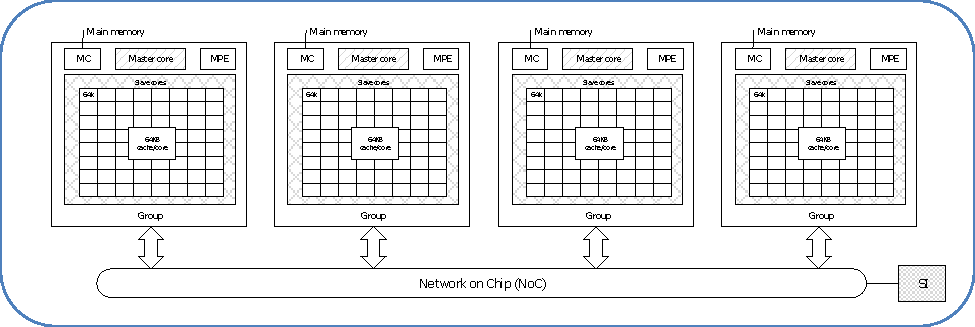
\includegraphics[scale=1]{\locpath/figures/Chap1/report_sunway_CPE}
\caption{Sunway Taihulight node architecture from \textit{Report on the Sunway TaihuLight System}, Jack Dongarra, June 24, 2016.}
\label{fig:chap1_report_sunway_CPE}
\end{figure}

The SW26010, a many core architecture processor, features 260 cores based on RISC architecture and a specific conception depicted on figure~\ref{fig:chap1_report_sunway_CPE}. 
The processor is composed of the master core, a Memory Controller (MC), a Management Processing Element (MPE) that manages the Computing Processing Elements (CPE) which are the slaves cores. 

The interconnect network is called Sunway Network and connected using Mellanox Host Channel Adapter (HCA) and switches. 
This is a five level interconnect going through computing nodes, computing board, super-nodes and cabinets to the complete system.
The total memory is 1.31 PB and the number of cores available is 10,649,600.
The peak performance is 125.4 PFLOPS and the Linpack is 93 PFLOPS which induce 74.16\% of efficiency. 

\subsubsection{Piz Daint}
\index{Piz Daint}
The supercomputer of the CSCS, Swiss National Supercomputing Center, is currently ranked 2nd of the November 2017 TOP500 list. 
This GPUs accelerated supercomputer is a most powerful representative of GPU hybrid acceleration.
This is also the most powerful European supercomputer. 
He is composed of 4761 hybrids and 1210 multi-core nodes. 
\index{NVIDIA}
The hybrids nodes embedded an Intel Xeon E5-2690v3 and an NVIDIA Tesla Pascal P100 GPGPU. 
The interconnect is based on a Dragonfly network topology and Cray Aries routing and communications ASICs. 
The peak performance is 25.326 TFLOPS using only the hybrid nodes and the Linpack gives 19.590 TFLOPS.
The low power consumption rank Piz Daint as 10th in the GREEN500 list. 

\subsubsection{K-Computer}
\index{K-Computer}
K-Computer was the top 1 supercomputer of TOP500 2011 list. 
The TOFU interconnect network makes the K-Computer unique~\cite{ajima2009tofu} and stands for TOrus FUsion.
\begin{figure}[t!]
\begin{center}
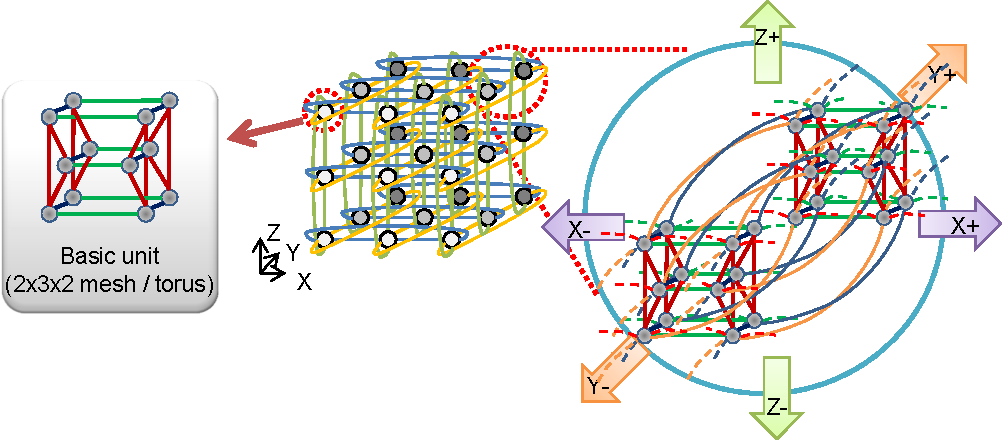
\includegraphics[width=\textwidth]{\locpath/figures/chap1/6d_torus}
\end{center}
\caption{TOFU Interconnect schematic from \textit{The K-Computer: System Overview}, Atsuya Uno, SC11}
\label{fig:1_HPC:tofu}
\end{figure}
\index{Interconnection}
This interconnect presented in figure~\ref{fig:1_HPC:tofu} mixes a 6D Mesh/Torus interconnect.
The basic units are based on a mesh and are interconnected together in a 3 dimensional torus. 
In this configuration each node can access to its 12 neighbors directly. 
It also provide a fault tolerant network with many routes to reach distant node. 

%\todo{AJouter MIRA/SEQUOIA pour paler de IBM, pour le Graph500 = meilleurs supercomputers}
%\todo{Parler de CRAY ?}
\subsubsection{Sequoia/Mira}
\index{IBM BlueGene}
Sequoia supercomputer was top 1 of the TOP500 2012 list. 
It is based on BlueGene from IBM.
The BlueGene project made up to three main architectures with BlueGene/L, BlueGene/P and BlueGene/Q.
It is very interesting to notice the BlueGene architecture because even in the last GRAPH500 list, November 2017, there is 15 of these machines in the TOP20.
The algorithm used on these supercomputers will be our basis in the part II regarding our implementation of the GRAPH500 benchmark.

\section{ROMEO Supercomputer}
\index{ROMEO Supercomputer}
The ROMEO supercomputer center is the computation center of the Champagne-Ardenne region in France. 
Hosted since 2002 by the University of Reims Champagne-Ardenne, this so called meso-center (French name for software and hardware architectures) is used for HPC for theoretic research and domain science like applied mathematics, physics, biophysics and chemistry. 

This project is support by the Champagne-Ardenne region and the CEA (French Alternative Energies and Atomic Energy Commission), aim to host research and production codes of the region for industrial, research and academics purposes. 

We are currently working on the third version of ROMEO, installed in 2013. 
As many of our tests in this study have been done on this machine, we will carefully describe its architecture. 

This supercomputer was ranked 151st in the TOP500 and 5th in the GREEN500 list. 

\subsection{ROMEO hardware architecture}
\label{sec:part1_ROMEO}
ROMEO is a Bull/Atos supercomputer composed of 130 BullX R421 computing nodes. 

\index{K20Xm}
Each node is composed of two processors Intel Ivy Bridge 8 cores @ 2,6 GHz. 
Each processor have access to 16GB of memory for a total of 32GB per node, the total memory if 4.160TB. 
Each processor if linked, using PCIe-v3, to an NVIDIA Tesla K20Xm GPGPU. 
This cluster provide then 260 processors for a total of 2080 CPU cores and 260 GPGPU providing 698880 GPU cores. 
The computation nodes are interconnected with an Infiniband QDR non-blocking network structured as a FatTree. 
The Infiniband is a QDR providing 10GB/s. 

The storage for users is 57 TB and the cluster also provide 195 GB of Lustre and 88TB of parallel scratch file-system. 

In addition to the 130 computations nodes, the cluster provides a visualization node NVIDIA GRID with two K2 cards and 250GB of DDR3 RAM. 
The old machine, renamed Clovis, is always available but does not features GPUs. 

The supercomputer supports MPI with GPU Aware and GPUDirect. 

\subsection{New ROMEO supercomputer, June 2018}
\todo{Avoir les info et decrire le nouveau ROMEO}


\section{Conclusion}

In this chapter we reviewed the most important nowadays hardware architectures and technologies. 
In order to use the driver or API in the most efficient way we need to keep in mind the way the data and instructions are proceed by the machine. 

As efficiency is based on computation power but also communications we showed different interconnection topologies and their specificities. 
We presented perfect use cases of the technologies in nowadays top ranked systems.
They also show that every architecture is unique in its construction and justify the optimization work dedicated to reach performance. 

We can see through the new technologies presented here that every one is moving toward hybrids architectures featuring multi-core processors accelerated by one or more devices, many-core architectures. 
The exascale supercomputer of 2020 will be shape with hybrid architectures and they represent the best of nowadays technology for purpose of HPC. 
Combining CPU and GPUs or FPGA on the same die, sharing the same memory space can also be the solution.
